\documentclass[twoside,11pt]{article}
\usepackage{graphicx}
% \usepackage[draft]{graphicx}
\pagestyle{myheadings}

% -----------------------------------------------------------------------------
% ? Document identification - generic part
\newcommand{\stardoccategory}  {Starlink User Note}
\newcommand{\stardocinitials}  {SUN}
\newcommand{\stardocsource}    {sun\stardocnumber}
% -----------------------------------------------------------------------------
% ? Document identification - document specific part
% \newcommand{\stardocnumber}    {251.1 -- Draft}
\newcommand{\stardocnumber}    {251.1}
\newcommand{\stardocauthors}   {S.\,E.\,Rankin}
\newcommand{\stardocdate}      {29 July 2003}
\newcommand{\stardoctitle}     {Getting Started with the Starlink Java Infrastructure and Applications Set}
\newcommand{\stardocversion}   {V1.0b}
\newcommand{\stardocmanual}    {}
\newcommand{\stardocabstract}  {}

% ? End of document identification

% -----------------------------------------------------------------------------

\newcommand{\stardocname}{\stardocinitials /\stardocnumber}
\markboth{\stardocname}{\stardocname}
\setlength{\textwidth}{160mm}
\setlength{\textheight}{230mm}
\setlength{\topmargin}{-2mm}
\setlength{\oddsidemargin}{0mm}
\setlength{\evensidemargin}{0mm}
\setlength{\parindent}{0mm}
\setlength{\parskip}{\medskipamount}
\setlength{\unitlength}{1mm}

% -----------------------------------------------------------------------------
%  Hypertext definitions.
%  ======================
%  These are used by the LaTeX2HTML translator in conjunction with star2html.

%  Comment.sty: version 2..0, 19 June 1992
%  Selectively in/exclude pieces of text.
%
%  Author
%    Victor Eijkhout                                      <eijkhout@cs.utk.edu>
%    Department of Computer Science
%    University Tennessee at Knoxville
%    104 Ayres Hall
%    Knoxville, TN 37996
%    USA

%  Do not remove the %begin{latexonly} and %end{latexonly} lines (used by 
%  LATEX2HTML to signify text that it shouldn't process).
%begin{latexonly}
\makeatletter
\def\makeinnocent#1{\catcode`#1=12 }
\def\csarg#1#2{\expandafter#1\csname#2\endcsname}

\def\ThrowAwayComment#1{\begingroup
    \def\CurrentComment{#1}%
    \let\do\makeinnocent \dospecials
    \makeinnocent\^^L% and whatever other special cases
    \endlinechar`\^^M \catcode`\^^M=12 \xComment}
{\catcode`\^^M=12 \endlinechar=-1 %
 \gdef\xComment#1^^M{\def\test{#1}
      \csarg\ifx{PlainEnd\CurrentComment Test}\test
          \let\html@next\endgroup
      \else \csarg\ifx{LaLaEnd\CurrentComment Test}\test
            \edef\html@next{\endgroup\noexpand\end{\CurrentComment}}
      \else \let\html@next\xComment
      \fi \fi \html@next}
}
\makeatother

\def\includecomment
 #1{\expandafter\def\csname#1\endcsname{}%
    \expandafter\def\csname end#1\endcsname{}}
\def\excludecomment
 #1{\expandafter\def\csname#1\endcsname{\ThrowAwayComment{#1}}%
    {\escapechar=-1\relax
     \csarg\xdef{PlainEnd#1Test}{\string\\end#1}%
     \csarg\xdef{LaLaEnd#1Test}{\string\\end\string\{#1\string\}}%
    }}

%  Define environments that ignore their contents.
\excludecomment{comment}
\excludecomment{rawhtml}
\excludecomment{htmlonly}

%  Hypertext commands etc. This is a condensed version of the html.sty
%  file supplied with LaTeX2HTML by: Nikos Drakos <nikos@cbl.leeds.ac.uk> &
%  Jelle van Zeijl <jvzeijl@isou17.estec.esa.nl>. The LaTeX2HTML documentation
%  should be consulted about all commands (and the environments defined above)
%  except \xref and \xlabel which are Starlink specific.

\newcommand{\htmladdnormallinkfoot}[2]{#1\footnote{#2}}
\newcommand{\htmladdnormallink}[2]{#1}
\newcommand{\htmladdimg}[1]{}
\newcommand{\hyperref}[4]{#2\ref{#4}#3}
\newcommand{\htmlref}[2]{#1}
\newcommand{\htmlimage}[1]{}
\newcommand{\htmladdtonavigation}[1]{}

\newenvironment{latexonly}{}{}
\newcommand{\latex}[1]{#1}
\newcommand{\html}[1]{}
\newcommand{\latexhtml}[2]{#1}
\newcommand{\HTMLcode}[2][]{}

%  Starlink cross-references and labels.
\newcommand{\xref}[3]{#1}
\newcommand{\xlabel}[1]{}

%  LaTeX2HTML symbol.
\newcommand{\latextohtml}{\LaTeX2\texttt{HTML}}

%  Define command to re-centre underscore for Latex and leave as normal
%  for HTML (severe problems with \_ in tabbing environments and \_\_
%  generally otherwise).
\renewcommand{\_}{\texttt{\symbol{95}}}

% -----------------------------------------------------------------------------
%  Debugging.
%  =========
%  Remove % on the following to debug links in the HTML version using Latex.

% \newcommand{\hotlink}[2]{\fbox{\begin{tabular}[t]{@{}c@{}}#1\\\hline{\footnotesize #2}\end{tabular}}}
% \renewcommand{\htmladdnormallinkfoot}[2]{\hotlink{#1}{#2}}
% \renewcommand{\htmladdnormallink}[2]{\hotlink{#1}{#2}}
% \renewcommand{\hyperref}[4]{\hotlink{#1}{\S\ref{#4}}}
% \renewcommand{\htmlref}[2]{\hotlink{#1}{\S\ref{#2}}}
% \renewcommand{\xref}[3]{\hotlink{#1}{#2 -- #3}}
%end{latexonly}
% -----------------------------------------------------------------------------
% ? Document specific \newcommand or \newenvironment commands.

\newcommand{\cdrom}{CD--ROM}
\begin{htmlonly}
\newcommand{\cdrom}{CD-ROM}
\end{htmlonly}

\newcommand{\cdroms}{CD--ROMs}
\begin{htmlonly}
\newcommand{\cdroms}{CD-ROMs}
\end{htmlonly}

\newcommand{\latexonlysmall}{\small}
\begin{htmlonly}
   \newcommand{\latexonlysmall}{}
\end{htmlonly}

% ? End of document specific commands
% -----------------------------------------------------------------------------
%  Title Page.
%  ===========
\renewcommand{\thepage}{\roman{page}}
\begin{document}
\thispagestyle{empty}

%  Latex document header.
%  ======================
\begin{latexonly}
   CCLRC / \textsc{Rutherford Appleton Laboratory} \hfill \textbf{\stardocname}\\
   {\large Particle Physics \& Astronomy Research Council}\\
   {\large Starlink Project\\}
   {\large \stardoccategory\ \stardocnumber}
   \begin{flushright}
   \stardocauthors\\
   \stardocdate
   \end{flushright}
   \vspace{-4mm}
   \rule{\textwidth}{0.5mm}
   \vspace{5mm}
   \begin{center}
   {\Huge\textbf{\stardoctitle \\ [2.5ex]}}
   {\LARGE\textbf{\stardocversion \\ [4ex]}}
   {\Huge\textbf{\stardocmanual}}
   \end{center}
   \vspace{5mm}

% ? Add picture here if required.
%\centering 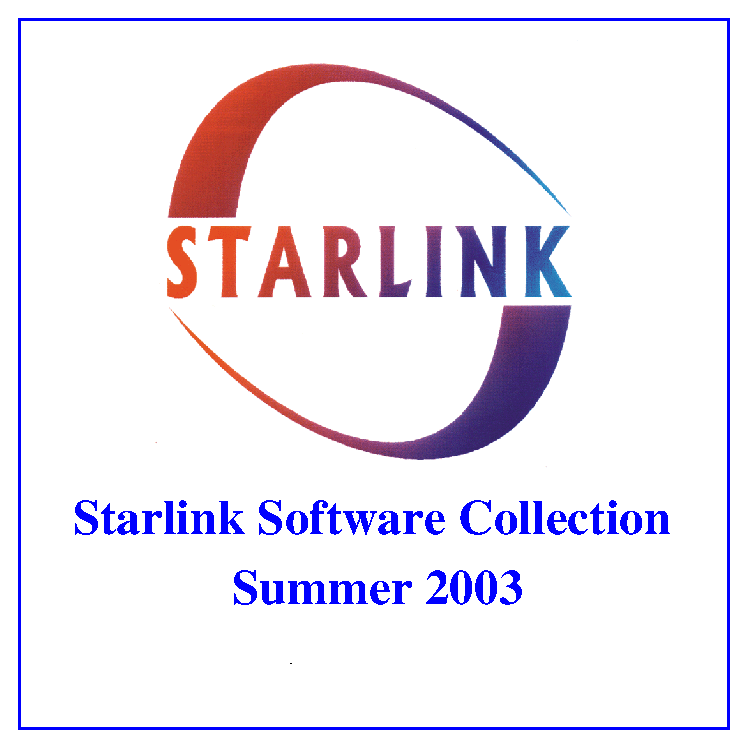
\includegraphics[scale=1.0]{sun212_cover.eps}
% ? End of picture

% ? Heading for abstract if used.
%  \vspace{10mm}
%  \begin{center}
%     {\Large\textbf{Abstract}}
%  \end{center}
% ? End of heading for abstract.

\end{latexonly}

%  HTML documentation header.
%  ==========================
\begin{htmlonly}
   \xlabel{}
   \begin{rawhtml} <H1> \end{rawhtml}
      \stardoctitle\\
      \stardocversion\\
      \stardocmanual
   \begin{rawhtml} </H1> <HR> \end{rawhtml}

% ? Add picture here if required.
%  \begin{figure}[h]
%  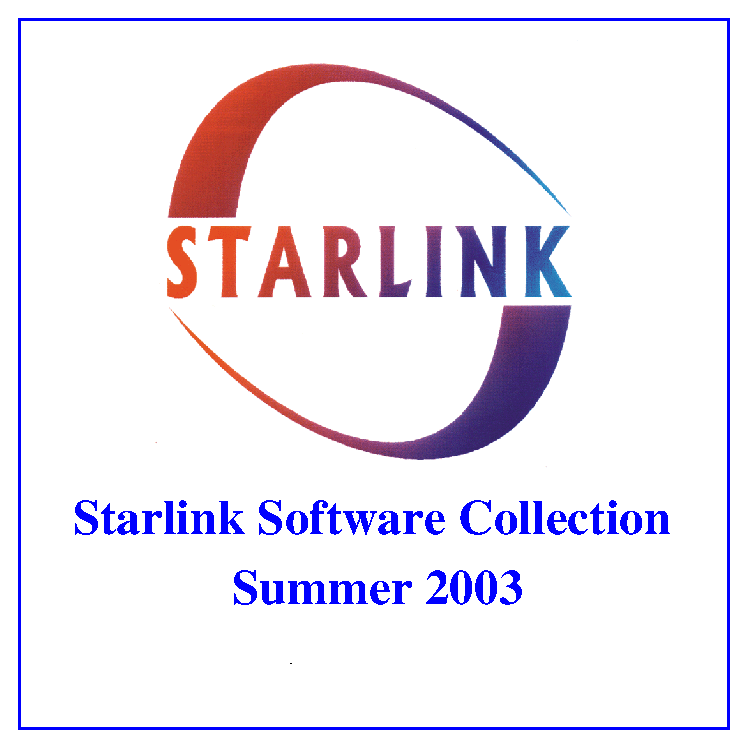
\includegraphics[scale=0.7]{sun212_cover.eps}
%  \end{figure}
% ? End of picture

   \begin{rawhtml} <P> <I> \end{rawhtml}
   \stardoccategory\ \stardocnumber \\
   \stardocauthors \\
   \stardocdate
   \begin{rawhtml} </I> </P> <H3> \end{rawhtml}
      \htmladdnormallink{CCLRC / Rutherford Appleton Laboratory}
                        {http://www.cclrc.ac.uk} \\
      \htmladdnormallink{Particle Physics \& Astronomy Research Council}
                        {http://www.pparc.ac.uk} \\
   \begin{rawhtml} </H3> <H2> \end{rawhtml}
      \htmladdnormallink{Starlink Project}{http://www.starlink.ac.uk/}
   \begin{rawhtml} </H2> \end{rawhtml}
   \htmladdnormallink{\htmladdimg{source.gif} Retrieve hardcopy}
      {http://www.starlink.ac.uk/cgi-bin/hcserver?\stardocsource}\\

%  HTML document table of contents. 
%  ================================
%  Add table of contents header and a navigation button to return to this 
%  point in the document (this should always go before the abstract \section). 
  \label{stardoccontents}
  \begin{rawhtml} 
    <HR>
    <H2>Contents</H2>
  \end{rawhtml}
  \htmladdtonavigation{\htmlref{\htmladdimg{contents_motif.gif}}
        {stardoccontents}}

% ? New section for abstract if used.
% \section{\xlabel{abstract}Abstract}
% ? End of new section for abstract
\end{htmlonly}

% -----------------------------------------------------------------------------
% ? Document Abstract. (if used)
%  ==================
% \stardocabstract
% ? End of document abstract
% -----------------------------------------------------------------------------
% ? Latex document Table of Contents (if used).
%  ===========================================
  \newpage
  \begin{latexonly}
     \setlength{\parskip}{0mm}
     \tableofcontents
     \setlength{\parskip}{\medskipamount}
     \markboth{\stardocname}{\stardocname}
  \end{latexonly}
% ? End of Latex document table of contents
% -----------------------------------------------------------------------------

% ==============================================================================
% PART 1 - GENERAL
% ==============================================================================

\cleardoublepage
\renewcommand{\thepage}{\arabic{page}}
\setcounter{page}{1}

\begin{latexonly}
\markright{\stardocname}
\end{latexonly}
%\part[The Summer 2003 Software \cdroms] %%
%{\label{version_of_cdrom}\xlabel{version_of_cdrom} %%
%The Summer 2003 Software \cdroms}
%\markboth{\stardocname}{\stardocname}

\section{\label{introduction}\xlabel{introduction}Introduction - Starlink Java Data Reduction and Analysis Software}
 
Starlink is developing a set of Java data reduction and analysis tools 
and Java data access classes. The new Java tools and classes are needed 
to produce applications in the Virtual Observatory (VO) era, and to 
complement the AstroGrid and other VO capabilities such as the International Virtual 
Observatory Alliance Data Model.

You can view a section of a proposed International Virtual Observatory 
Alliance Data Model, including HDX, NDX and Table data structures with 
the WCS astrometry library at

%\latex{\texttt{http://www.starlink.rl.ac.uk/java/java.htm}}

\htmladdnormallink{\texttt{http://www.starlink.rl.ac.uk/java/java.htm}}{http://www.starlink.rl.ac.uk/java/java.htm}

\section{\label{environment}\xlabel{environment}The Starlink Environment and Login Scripts}

In order to use the software the user should be using the JRE, this applies to both Windows 
and Unix versions. There are C-shell scripts (Unix only) to facilitate use of STARJAVA. 
If you are using the full Starlink Software Collection the standard Starlink login scripts, 
\texttt{login} and \texttt{cshrc} found in \texttt{/star/etc} will setup the required aliases 
and environment variables needed to run the software: 

\begin{quote}
\begin{verbatim}
% source /star/etc/login
% source /star/etc/cshrc
\end{verbatim}
\end{quote}

The STARJAVA package has its own \texttt{login} and \texttt{cshrc} files found in 
\texttt{/star/starjava/etc} which only initialise the Java Software, these need to be sourced:

\begin{quote}
\begin{verbatim}
% source /star/starjava/etc/login
% source /star/starjava/etc/cshrc
\end{verbatim}
\end{quote}

The Starlink Software Collection is now available on your machine and
can be run in the usual manner.

To run the Windows version of STARJAVA see \latex{(section~\ref{windows})} below.

\subsection{\label{Requirements}\xlabel{Requirements}Requirements for Running STARJAVA}

STARJAVA needs the SUN Java Runtime Environment (JRE) and optionally the Java
Advanced Imaging JAI packages, both are supplied on the Starlink Summer 2003 CD-ROM
as the JRE package. Currently the JRE is at version 1.4.1\_02, and the JAI at 
version 1\_1\_2-rc. Additionally some native code is required (JNIAST and JNIHDS),
but these are included in the distribution and are automatically installed. The 
following table shows the applications and their dependencies:
\pagebreak
\begin{quote}
\begin{verbatim}
             JRE1.4   JNIAST/JNIHDS             JAI
                      (Linux,Solaris,Windows)

   FROG           Y        Y
   SPLAT          Y        Y
   SoG            Y        Y                     Y
   Tablecopy      Y
   TOPCAT         Y
   Treeview       Y        *                     *

  Y: does require it
  *: will run without it, but with reduced functionality
\end{verbatim}
\end{quote}

If you experience problems with JRE v1.4.1\_02 distributed with
RedHat 9.0 CD, such as problems with the Java Plugin for Mozilla,
or Java crashes (SIGSEGV). Then a possible
cure is to set the environment variable \texttt{LD\_ASSUME\_KERNEL},

\begin{quote}
\begin{verbatim}
% setenv LD_ASSUME_KERNEL 2.4.1
\end{verbatim}
\end{quote}

\subsection{\label{windows}\xlabel{windows}STARJAVA for Microsoft Windows}

There is a Microsoft Windows version of STARJAVA which can be downloaded from \\
\htmladdnormallink{\texttt{ftp://ftp.starlink.ac.uk/pub/ussc/windows/starjava.exe}}{ftp://ftp.starlink.ac.uk/pub/ussc/windows/starjava.exe} 
and is also included on the Starlink CD-ROM in directory \texttt{windows}. 
To install STARJAVA just run the executable and you will be presented with a standard 
Windows graphical installer. You will have the options to install all applications and 
documentation, plus the Java Runtime Environment (JRE) and Java Advanced Imaging (JAI). 
JRE and JAI have their own installers, but these are started by the STARJAVA installer 
(if they are selected for installation). A full installation of everything is approximately 
191 Mb. You will also be presented with the option to select the installation directory.
Desktop icons (optional) and Start Menu Icons will be created with links to the 
GUI applications and documentation.

The Tablecopy program in the STARJAVA software can only be run from the 
Command Prompt (MS-DOS prompt),  

\begin{quote}
\begin{verbatim}
c:\> java -jar c:\path\to\starjava\lib\table\table.jar -help
\end{verbatim}
\end{quote}
 
A full explanation of the command line switches are given in \latex{(section~\ref{topcat})} of 
this document. The installation path \texttt{$c:\backslash path \backslash to \backslash starjava$} defaults to
\texttt{$c:\backslash Program \, Files \backslash starjava$}, substitute your install path if you have chosen it
to be something different during installation.

All the applications in STARJAVA can be run from the command line in a similar 
manner, details are given in this document. All switches indicated when describing
the Unix versions apply to the Windows version.

\subsection{\label{cdrom}\xlabel{cdrom}Running STARJAVA from the CD-ROM}

STARJAVA can be run from the CD-ROM if you have the Java Runtime 
Environment (JRE) v1.4 (or greater) and Java Advanced Imaging (JAI)
1.1\_2-rc (or greater) installed. The software will still run without 
the JAI but with reduced functionality. All the files in the distribution 
of STARJAVA are in the directory \texttt{starjava} on the CD-ROM.
Running the software from the CD-ROM will work for the Solaris, Linux
and Windows operating systems. There are five applications
that you can run, SOG, SPLAT, FROG, TREEVIEW and TABLECOPY. To run
the applications you need to supply the \texttt{jar} filename for
the application to the \texttt{java} command: 

\begin{quote}
\begin{verbatim}
For Unix

% java -jar /path/to/cdrom/starjava/lib/sog/sog.jar           (SOG)
% java -jar /path/to/cdrom/starjava/lib/splat/splat.jar       (SPLAT)
% java -jar /path/to/cdrom/starjava/lib/frog/frog.jar         (FROG)
% java -jar /path/to/cdrom/starjava/lib/treeview/treeview.jar (TREEVIEW)
% java -jar /path/to/cdrom/starjava/lib/table/table.jar       (TABLECOPY)
\end{verbatim}
\end{quote}

\texttt{/path/to/cdrom/} is the path to the top level of your mounted CD-ROM.

\begin{quote}
\begin{verbatim}
For Windows

c:\> java -jar D:\starjava\lib\sog\sog.jar           (SOG)
c:\> java -jar D:\starjava\lib\splat\splat.jar       (SPLAT)
c:\> java -jar D:\starjava\lib\frog\frog.jar         (FROG)
c:\> java -jar D:\starjava\lib\treeview\treeview.jar (TREEVIEW)
c:\> java -jar D:\starjava\lib\table\table.jar       (TABLECOPY)
\end{verbatim}
\end{quote}
\texttt{D:} is the letter of your CD-ROM drive.

The \texttt{java} command must be on your path for any of these commands to work.
See the rest of this document for further details on command
line switches that can be used with the applications.

\subsection{\label{development}\xlabel{development}Development with STARJAVA}

If you would like to do development with the STARJAVA API then you need to
obtain the Java Development Kit (JDK) for Microsoft Windows or the appropriate
Unix version. It can be downloaded from Sun's web site at:

\htmladdnormallink{\texttt{http://java.sun.com/products/archive/j2se/1.4.1\_02/index.html}}{http://java.sun.com/products/archive/j2se/1.4.1\_02/index.html}

This cannot be distributed by Starlink.

\section{\label{Applications}\xlabel{Applications}Applications and Utilities} 

\subsection{\label{treeview}\xlabel{treeview}TREEVIEW}

TREEVIEW is a graphical browser for hierarchical data structures written 
in Java. It knows about Starlink NDF and HDS data structures, as well 
as many other types of data such as file systems, zip and jar files, XML 
documents, FITS files and VO Tables. TREEVIEW is under active development,
see 
\htmladdnormallink{\texttt{http://www.starlink.ac.uk/treeview}}{http://www.starlink.ac.uk/treeview}
for the latest information.


\subsubsection{\label{features}\xlabel{features}List of features}

Treeview deals with the following generic forms of node:

\begin{itemize}
\item Arrays:
      These are found within FITS SIMPLE/IMAGE HDUs, Starlink HDS/NDF files
      and Starlink NDX structures, and represent an $N$-dimensional hypercube 
      of numbers. They have the following views:

\begin{itemize}
\item 1-d arrays (e.g. spectra) can be displayed as a line plot.
\item 2-d arrays can be displayed as an image at 1x magnification; this 
      does not require loading the whole image, so can be fast even for 
      large arrays.
\item The values of the pixels in even very large arrays can be viewed in a 
      scrollable 1-d or 2-d table. Again, the whole array does not need to be 
      loaded, so this is fast.
\item Higher-dimensional ($>$2d) arrays can be shown as image slices through the 
      array along any axis.
\item Three-dimensional arrays can be viewed collapsed (by averaging over some or 
      all planes) along any given axis to give an image.
\item Statistics (mean, variance etc) of an array can be calculated.
\item An external program SPLAT can be launched for detailed analysis of 1-d spectral data An 
      external program SoG can be launched for detailed inspection of 2-d image
      data. 
\end{itemize}

\item Tables: These are found in a variety of formats including TABLE/BINTABLE
      FITS extensions and VOTable files (more formats will be supported soon). 
      They have the following views:

\begin{itemize}
 \item Table data is shown in a compact scrollable table.
 \item Table has full JTable functionality - columns can be moved around,
       widths altered etc.
 \item All available column and table metadata can be displayed in a tabular
       format.
 \item An external program TOPCAT can be launched for detailed examination of
       the table. 
\end{itemize}

\item Treeview understands the structure of the following kinds of nodes and can display 
      them hierarchically:

\begin{itemize}

\item FITS files:

\begin{itemize}
 \item Each Header+Data Unit (HDU) in the FITS file is displayed.
 \item FITS header cards are displayed.
 \item BLANK values and BSCALE/BZERO scaling are handled properly.
 \item Simple FITS files and IMAGE, TABLE and BINTABLE extensions are
       recognised.
 \item All array views described above are supported for SIMPLE/IMAGE HDUs.
 \item All table views described above are supported for TABLE/BINTABLE HDUs.
 \item WCS information can be read from headers using a variety of encodings.
 \item WCS information can be plotted over image pixels or showing array extent
       for 2-d images.
 \item WCS information can be displayed in different FITS/non-FITS encodings. 
\end{itemize}

\item Starlink NDF files:

\begin{itemize}
 \item All array views described above are supported.
 \item Magic bad values are treated properly.
 \item The co-ordinate Frames can be viewed in several formats (native, XML and a 
       variety of FITS encodings).
 \item The extent of a 2-d array in any of its WCS co-ordinate Frames can be displayed, 
       with a grid plotted.
 \item NDF HISTORY components are shown. 
\end{itemize}

\item Starlink HDS container files:
\begin{itemize}
 \item The structure of arbitrarily complicated HDS files can be seen.
 \item All array views described above are supported for array components. 
\end{itemize}

\item VOTable files:
\begin{itemize}
 \item Compact display of complicated VOTable structures.
 \item Most aspects of VOTable hierarchical structure are understood.
 \item All FIELD and PARAM metadata can be viewed in a tabular form.
 \item TABLEDATA, FITS and (so far untested) BINARY table data support.
 \item Relative or absolute, local or network URLs for FITS files.
 \item XML content of any VOTable element can be seen.
 \item VOTable DTD stored locally for standalone operation. 
\end{itemize}

\item XML documents:
\begin{itemize}
 \item Hierarchical view of XML documents.
 \item Summary or full display of each node can be seen.
 \item Known structures (NDX, VOTable) embedded in larger documents are
       recognised.
 \item Many standard XML encodings supported. 
\end{itemize}

\item Zip files:
\begin{itemize}
 \item Zip (PKZIP-like) and Jar archives displayed like directory structures.
 \item Many node types within archive can be viewed as if they were normal
       files. 
\end{itemize}

\item Tar files:
\begin{itemize}
 \item Tar archives displayed like directory structures.
 \item Many node types within archive can be viewed as if they were normal
       files. 
\end{itemize}

\item Starlink NDX structures:
\begin{itemize}
 \item NDFs, FITS files and suitable XML files can be viewed as NDXs or as
       their native type.
 \item All array views described above are supported.
 \item WCS information can be plotted over image pixels or showing array extent
       for 2-d images.
 \item WCS information can be displayed in various formats (XML, FITS, AST). 
\end{itemize}

\item Starlink HDX containers:
\begin{itemize}
 \item Hierarchical view of contained resources.
 \item XML view can be seen. 
\end{itemize}

\item Directories:
\begin{itemize}
 \item Hierarchical view of file systems. 
\end{itemize}

\item Files:
\begin{itemize}
 \item Hex dump or text content of file can be shown.
 \item File system information is displayed. 
\end{itemize}

\item  Compressed data:
\begin{itemize}
 \item Files compressed in \texttt{gzip} or \texttt{bzip2} format can be viewed.
 \item Hex dump or text of uncompressed content can be shown. 
\end{itemize}
\end{itemize}

\item Other features:
\begin{itemize}
 \item Basic on-line help system.
 \item Popup `alter-ego' menus allow nodes to be seen in different aspects 
      (e.g. view a VOTable as an XML document) or reloaded to reflect change of 
      underlying data.
 \item Demonstration data is integral to the tool and can be viewed at any time to 
       investigate Treeview capabilities. 
\end{itemize}      
\end{itemize}

Support Page at 
%\latex{\texttt{http://www.starlink.ac.uk/treeview}}
\htmladdnormallink{\texttt{http://www.starlink.ac.uk/treeview}}{http://www.starlink.ac.uk/treeview}

Documentation for Treeview is available in the form of online help 
in the program itself.

Treeview can be run from the shell prompt (when the Starlink login scripts have 
been sourced, see above) by typing treeview with the name of a
file you would like to look at:

\begin{quote}
\begin{verbatim}
% treeview [file ...]
\end{verbatim}
\end{quote}

or simply just

\begin{quote}
\begin{verbatim}
% treeview
\end{verbatim}
\end{quote}

and for Windows

\begin{quote}
\begin{verbatim}
c:\> java -jar c:\path\to\starjava\lib\treeview\treeview.jar
\end{verbatim}
\end{quote}

\subsection{\label{splat}\xlabel{splat}SPLAT}

SPLAT is a graphical tool for displaying, comparing, modifying and analysing 
astronomical spectra stored in NDF, FITS and TEXT files as well as the new 
NDX format. 

SPLAT can read in many spectra at the same time and then display these 
as line plots. Each display window, of which there can be many, can be used to 
view one or several spectra at the same time. Display windows can be interactively 
zoomed and scrolled, centered on specific wavelengths, provide continuous 
coordinate readout, produce printable hardcopy and be configured in many ways. 
They also provide the basis for interactive analysis facilities. All of these 
functions are displayed in a visually rich format, that is intended to appeal 
especially to casual users of spectral data analysis facilities, as it includes 
some facilities such as drag-and-drop and undoable editing.

The current set of analysis facilities include the fitting of a polynomial to 
selected parts of a spectrum, the fitting of Gaussian, Lorentzian and Voigt profiles 
to emission and absorption lines and the filtering of spectra using average, median 
and line-shape window functions as well as wavelet denoising. A database of laboratory 
line positions is available to aid in identification.

SPLAT also supports a full range of coordinate systems for spectra, using the 
latest facilities of the Starlink AST library. This allows coordinates to be 
displayed and aligned in many different coordinate systems (wavelength, frequency, 
energy, velocity) and transformed between these and different standards of rest 
(topocentric, heliocentric, dynamic and kinematic local standards of rest etc.).

If you have any problems with or comments to make about SPLAT then send \\
these to
\htmladdnormallink{texttt{splat@star.rl.ac.uk}}{splat@star.rl.ac.uk}.

\subsubsection{Documentation}

The main source of documentation for SPLAT is Starlink User Note 243 
\xref{SPLAT}{sun243}{}, which is 
also the on-line help. If you have SPLAT installed on your machine then you 
should be able to view this using the `Help' menu. Otherwise (if you just 
want a look) you can find it on-line.

Initially you should work you way through the getting started, displaying more 
than one spectrum and basic control of a plot view sections.

SPLAT can be run from the shell prompt (when the Starlink login scripts have 
been sourced, see above) by typing splat with the name of a spectrum
file you would like to look at:

\begin{quote}
\begin{verbatim}
% splat <spectrum_file>
\end{verbatim}
\end{quote}

or simply just

\begin{quote}
\begin{verbatim}
% splat
\end{verbatim}
\end{quote}


and for Windows

\begin{quote}
\begin{verbatim}
c:\> java -jar c:\path\to\starjava\lib\splat\splat.jar
\end{verbatim}
\end{quote}


Support Page at 
%\latex{\texttt{http://www.starlink.ac.uk/splat}}
\htmladdnormallink{\texttt{http://www.starlink.ac.uk/splat}}{http://www.starlink.ac.uk/splat}


\subsection{\label{frog}\xlabel{frog}FROG}
FROG is a new graphical tool for displaying, comparing and 
analysing time series data.

See the support page for further information.

Support Page at 
%\latex{\texttt{http://www.starlink.ac.uk/frog}}
\htmladdnormallink{\texttt{http://www.starlink.ac.uk/frog}}{http://www.starlink.ac.uk/frog}

FROG can be run from the shell prompt (when the Starlink login scripts have 
been sourced, see above) by typing:

\begin{quote}
\begin{verbatim}
% frog
\end{verbatim}
\end{quote}

and for Windows

\begin{quote}
\begin{verbatim}
c:\> java -jar c:\path\to\starjava\lib\frog\frog.jar
\end{verbatim}
\end{quote}

\subsection{\label{sog}\xlabel{sog}SoG}
SoG - Son of GAIA - is an extension of ESO JSkycat which can display our 
new HDX/NDX format, as well as FITS and NDF images.

SoG and JSkycat implement a number features, which include:

\begin{itemize}
 \item Ability to load, save, print, and display images in FITS, JPEG, GIF, PNG, 
       and other formats
 \item Image operations (zoom, pan, manipulate the colormap, set cut levels, ...)
 \item World coordinates support
 \item Support for compressed FITS images (gzip, H-compress)
 \item Access local and web based astronomical catalogs and image servers
 \item Support for local catalogs and editing catalog tables
 \item Plot the results of catalog searches as image overlays
 \item Draw graphics interactively on the image
 \item Save graphics and catalog query results in FITS tables with the image, 
       for later redisplay
\end{itemize}

Using web-service interfaces it can be remotely controlled and used to 
display images (as it currently does from Starlink Treeview). In the 
fullness of time it is expected to provide similar features to GAIA 
(but working within the Grid).

See the support page for further information.

Support Page at 

%\latex{\texttt{http://www.starlink.ac.uk/sog}}
\htmladdnormallink{\texttt{http://www.starlink.ac.uk/sog}}{http://www.starlink.ac.uk/sog}

SoG can be run from the shell prompt (when the Starlink login scripts have 
been sourced, see above) by typing:

\begin{quote}
\begin{verbatim}
% sog
\end{verbatim}
\end{quote}

and for Windows

\begin{quote}
\begin{verbatim}
c:\> java -jar c:\path\to\starjava\lib\sog\sog.jar
\end{verbatim}
\end{quote}

\subsection{\label{topcat}\xlabel{topcat}TOPCAT} 

TOPCAT - Tool for OPerations on Catalogues and Tables, a viewer/editor for 
astronomical tabular data, including FITS table extensions and 
VOTable documents. TOPCAT is a viewer and editor for tabular information. 
It has been designed to be able to deal with large astronomical tabular data, 
but is not restricted to astronomical use. It can read and write a number of 
different astronomically important formats, including FITS tables, VOTable 
documents, relational databases such as ORACLE, and more formats will be added.

Here is a list of its main features:

\begin{itemize}
 \item View/edit table data in a scrollable browser
 \item View/edit table and column metadata
 \item Re-order or delete columns
 \item Insert 'synthetic' columns (algebraic expression)
 \item Sort rows on the values in a given column
 \item Define row subsets in various ways
 \item Plot columns against each other, distinguishing different subsets
 \item Calculate statistics on each column for some or all rows
 \item Write modified table out in original or different format
 \item Launch other programs (Mirage) 
\end{itemize}

Please note: TOPCAT is a new product under active development, and the 
             currently released version is beta software. 

Documentation for TOPCAT is available in the form of online help 
in the program itself.

Support Page at 
%\latex{\texttt{http://www.starlink.ac.uk/topcat}}
\htmladdnormallink{\texttt{http://www.starlink.ac.uk/topcat}}{http://www.starlink.ac.uk/topcat}

TOPCAT can be run from the shell prompt (when the Starlink login scripts have 
been sourced, see above) by typing:

\begin{quote}
\begin{verbatim}
% topcat
\end{verbatim}
\end{quote}

Invoked with no arguments, this will pop up the `\texttt{Open Table}' dialogue window.

Alternatively, you can supply command-line arguments giving the name(s) of one 
or more tables to load - filenames or URLs with optional fragment IDs following
a '\#' character, or JDBC table specifiers, for example

\begin{quote}
\begin{verbatim}
% topcat dsscat.xml
\end{verbatim}
\end{quote}

or

\begin{quote}
\begin{verbatim}
% topcat cat1.fits#1 cat1.fits#2 http://astro.org/data/m31.xml
\end{verbatim}
\end{quote}


and for Windows

\begin{quote}
\begin{verbatim}
c:\> java -jar c:\path\to\starjava\lib\topcat\topcat.jar
\end{verbatim}
\end{quote}


\subsection{\label{tablecopy}\xlabel{tablecopy}Tablecopy}

Tablecopy is a simple command-line tool for copying tables from
one format to another. If you have a normal Starlink installation it
can be invoked by just using the \texttt{tablecopy} command.
Supplying the \texttt{-help} flag gives its usage message:
\begin{verbatim}
   % tablecopy -help

      Usage: TableCopy [-ofmt jdbc|text|votable|fits|mirage] in-table out-table 

\end{verbatim}

and for Windows

\begin{quote}
\begin{verbatim}
c:\> java -jar c:\path\to\starjava\lib\table\table.jar -help
\end{verbatim}
\end{quote}

In general you give the name of the input file followed by the
name of the output file as command-line arguments.  The \texttt{-ofmt}
flag should also normally be used to determine the format of the
output table, but the tool will sometimes guess the format based
on the output filename given; for instance an output filename with
the extension `\texttt{.fits}' indicates a FITS file, and the extension `\texttt{.xml}'
indicates a VOTable.

In some cases the name of the output file can be given as `-' which
indicates that it should be written to standard output.
This can be used to see a table's contents at the terminal, 
such as that below.

\begin{verbatim}
   % tablecopy -ofmt text tables.fit#2 -
   +-------------+---------------+--------------+
   | FLUX        | DELTAX        | DELTAY       |
   +-------------+---------------+--------------+
   | 0.13405019  | -1.1666666E-5 | 8.3333333E-7 |
   | 0.12064518  | -1.1666666E-5 | 8.3333333E-7 |
   | 0.108580664 | -1.1666666E-5 | 8.3333333E-7 |
   | 0.0977226   | -1.1666666E-5 | 8.3333333E-7 |
       ....
\end{verbatim}

The same considerations apply to the input and output table names
and formats as for the TOPCAT application.
Full details can be found in TOPCAT's online help (which can be
invoked from within the package or with the
invocation `\texttt{topcat -guihelp}'),
but the following is a summary:

\subsubsection{\label{Input}\xlabel{Input}Input table}

The following describe the table formats which can 
be read (i.e. copied from).  In most cases the specified name
can be a URL or a filename, and may refer to a resource which has
been compressed using the \texttt{gzip} or \texttt{bzip2} formats.
The input format does not need to be specified, it is sensed automatically
from the named resource.

\begin{itemize}

\item FITS binary and ASCII tables can be read.  Unless otherwise specified,
the first TABLE or BINTABLE extension in the file will be used.
If a later extension is required, this is specified by giving the
extension number after a `\#' at the end of the table location.
The first extension (first HDU after the primary HDU) is numbered 1.
Thus in a compressed FITS table called `spec23.fits.gz'
with one primary HDU and two BINTABLE extensions,
you would view the first one using the name `spec23.fits.gz'
or `spec23.fits.gz\#1' and the second one using the name.
`spec23.fits.gz\#2'.  The suffix `\#0' is never used for a legal
FITS file, since the primary HDU cannot contain a table.

\item Any VOTable which conforms to the VOTable 1.0 specification should be
readable.
Unless otherwise specified, the first TABLE element found in the 
named document will be used, so in the (common) case that
the document holds exactly one table, giving the filename will
display that sole table.
To display a table other than the first, you must indicate the
zero-based index of the TABLE element in a breadth-first search
after a `\#' character at the end of the table specification.

Here is an example VOTable document:
\begin{verbatim}
  <VOTABLE>
    <RESOURCE>
      <TABLE name="Star Catalogue"> ... </TABLE>
      <TABLE name="Galaxy Catalogue"> ... </TABLE>
    </RESOURCE>
  </VOTABLE>
\end{verbatim}
If this is available in a file called `\texttt{cats.xml}', then the name
`\texttt{cats.xml}' or `\texttt{cats.xml\#0}' refers to the Star Catalogue, and
`\texttt{ccats.xml\#1}' refers to the Galaxy Catalogue.


\item Some support is provided for files produced by the World Data Centre
for Solar Terrestrial Physics based at the Rutherford Appleton Laboratory.
The format itself apparently has no name, but files in this format
look something like the following:
\begin{verbatim}
  Column formats and units - (Fixed format columns which are 
  single space seperated.)
  ------------------------
  Datetime (YYYY mm dd HHMMSS)            %4d %2d %2d %6d      -
                                          %1s
  aa index - 3-HOURLY (Provisional)       %3d                  nT

  2000 01 01 000000  67
  2000 01 01 030000  32
      ...
\end{verbatim}
This handler is experimental; it was reverse-engineered from looking
at a couple of example data files in the target format, and may
not be very robust.


\item With appropriate configuration, Tablecopy can access the 
results of queries on SQL compatible relational databases such as 
MySQL. This requires installation of an appropriate JDBC driver 
specific to that database as well as, of course, access to such a 
database locally or over a network. You will need to ensure that
the driver is installed by defining the `\texttt{jdbc.drivers}' property
appropriately and ensuring that the named Driver class is available 
from your classpath when running \texttt{tablecopy}.

Database queries have the form
\begin{verbatim}
  jdbc:<driver-specific-url>#<sql-query>
\end{verbatim}

See the TOPCAT help system for more detail on this topic.
\end{itemize}

\subsubsection{\label{output}\xlabel{output}Output table}

The following list describes the formats to which tablecopy
can write (i.e.\ copy to).  To ensure that you are writing in the right format,
use the appropriate `\texttt{-ofmt}' command-line flag.

\begin{itemize}

\item Using the `\texttt{-ofmt fits}' flag, a two-HDU FITS file is written.
The first (primary) HDU is a minimal dummy one, and the second is
a BINTABLE extension containing the table data.

\item Using the `\texttt{-ofmt votable}' flag, an XML file is written
which conforms to the VOTable DTD.  It will contain a single TABLE
element containing a TABLEDATA element.
Note that since this encodes all the data as in-line XML text elements,
it is not too suitable for very large tables (though such tables can
be written).

\item Using the `\texttt{-ofmt text}' flag, an ASCII representation of the
table data is written.  This is intended for human consumption rather
than as a machine-readable format, though if there are many columns
it may still be difficult to see what is going on.  The table and
column metadata (except for the column names themselves) are not
written in this case.

\item Using the `\texttt{-ofmt mirage}' flag will write to a format suitable for
use as input to the {\em Mirage\/} tool.
Mirage is a powerful standalone Java tool developed at Bell labs for
analysis of multidimensional data.  It uses its own file format for input.

\item Using the `\texttt{-ofmt jdbc}' flag can create a new table in a supported
SQL database if a suitable JDBC driver is installed.  The output resource
name has the form.
\begin{verbatim}
  jdbc:<driver-specific-url>\#<new-table-name>
\end{verbatim}

See the TOPCAT help system for more detail on this topic.
\end{itemize}

\section{\label{classes}\xlabel{classes}CLASSES}

\subsection{\label{native}\xlabel{native}Native Interfaces and HDX data model}

\begin{itemize}

\item JNIAST - a Java wrapper of the Starlink AST coordinate manipulation library.

Support Page at 
%\latex{\texttt{http://www.starlink.ac.uk/jniast}}
\htmladdnormallink{\texttt{http://www.starlink.ac.uk/jniast}}{http://www.starlink.ac.uk/jniast}

\item JNIHDS - a Java wrap of the Starlink HDS hierarchical data storage library.

Support Page at 
%\latex{\texttt{http://www.starlink.ac.uk/jnihds}}
\htmladdnormallink{\texttt{http://www.starlink.ac.uk/jnihds}}{http://www.starlink.ac.uk/jnihds}

\item HDX - a flexible, extensible, data model for astronomical images, tables and 
      other metadata; and a data access layer, consisting of Java packages 
      which handle the XML and URIs involved, and cast a variety of local 
      or network resources into the HDX data model.

Support Page at 
%\latex{\texttt{http://www.starlink.ac.uk/HDX}}
\htmladdnormallink{\texttt{http://www.starlink.ac.uk/HDX}}{http://www.starlink.ac.uk/HDX}

\end{itemize}

\subsection{\label{general}\xlabel{general}General Classes in STARJAVA}

Starlink Java Infrastructure - the next generation of Starlink 
astronomical data software. Much of this is still under active development, 
but it includes the ARRAY, AST, FITS, HDS, NDX, TABLE, TASK, UTIL and VOTABLE 
packages:

\begin{itemize}
\item ARRAY V0.2 $N$-dimensional array manipulation and I/O (new).
\item ASTGUI V1.0 AST specific UI components (new).
\item COCO V1.0 Java UI for Coco (new).
\item FITS V0.1 Starjava-specific FITS access (new).
\item HDS V0.1 Non-native HDS utility classes (new).
\item JAIUTIL V1.0 Utility classes for JAI (new).
\item NDX V0.1 $N$-dimensional astronomical object manipulation and I/O (new).
\item PAL V0.1 Positional Astronomy Library (new).
\item RV V1.0 Java UI for RV (new).
\item TABLE V0.3 Generic table manipulation and I/O (new).
\item UTIL V0.1 Miscellaneous utility classes (new).
\item VOTABLE V1.0 VOTable I/O (new).
\end{itemize}

Third party classes:

\begin{itemize}
\item AXIS V1.0b2 Third generation Apache SOAP (new).
\item DOM4J V0.1 Third party DOM access library (org.dom4j.*) (new).
\item JETTY V4.0.4 HTTP Server and Servlet Container (new).
\item JUNIT V3.7 Third party unit testing framework (junit.*) (new).
\item JSKY V2.0 Java Components for Astronomy (new)
\item TAMFITS V0.93 Third party basic FITS acccess (nom.tam.*) (new).
\end{itemize}

\subsection{\label{Javadocs}\xlabel{Javadocs}STARJAVA Class Documentation}

Javadocs for Starlink Java Classes can be seen at:

%\latex{\texttt{http://www.starlink.ac.uk/starjavadocs}}
\htmladdnormallink{\texttt{http://www.starlink.ac.uk/starjavadocs}}{http://www.starlink.ac.uk/starjavadocs}

%\latex{\texttt{/star/starjava/javadocs/index.html}}
or locally at

\htmladdnormallink{\texttt{file:///star/starjava/javadocs/index.html}}{file:///star/starjava/javadocs/index.html}

There are miscellaneous documents in \texttt{/star/starjava/docs/} for individual package information and
third party application documentation. Each subdirectory in
\texttt{/star/starjava/docs/} is named after the package and contains its documentation.


\section{\label{license}\xlabel{license}License and Source Code}

The above Java applications and classes are released under the GNU GPL 
licence. The source code CVS repository can be viewed via cvsweb at 

%\latex{\texttt{http://cvsweb.starlink.ac.uk}} .
\htmladdnormallink{\texttt{http://cvsweb.starlink.ac.uk}}{http://cvsweb.starlink.ac.uk}

Starlink has recently revised the conditions of use of the Starlink 
software. The software is still distributed free of distribution charge,
but is now under GPL Licence.

\begin{quote}
\latexonlysmall
\begin{center}\textbf{STARLINK SOFTWARE COPYRIGHT}\end{center}
 
\textbf{PREAMBLE}

The purpose of this document is to state the terms and conditions
under which Starlink software, documentation, data and other associated
material (``the Software'') may be used.

\par 
\textbf{NOTICE TO USER:}
\par 
\textbf{BY USING THE SOFTWARE YOU ACCEPT THE FOLLOWING TERMS AND CONDITIONS
WHICH APPLY TO ITS USE.}
 
\begin{enumerate}

\item The Starlink STARJAVA Software Collection is Copyright 1980-2003, Council 
 for the Central Laboratory of the Research Councils (``CCLRC''), 
 except where noted internally, or discussed below.

\item The Starlink Project has recently made the decision to license its
 own software under the GNU General Public License (GPL) as published 
 by the Free Software Foundation; either version 2 of the License, 
 or (at your option) any later version.

\item If you wish to use the code for a purpose for which the licence
 conditions, authorship or copyright are important, you should 
 consult the project at \htmladdnormallink{ussc@star.rl.ac.uk}{mailto:ussc@star.rl.ac.uk}

\item This Software is distributed in the hope that it will be useful, but 
 WITHOUT ANY WARRANTY; without even the implied warranty of 
 MERCHANTABILITY or FITNESS FOR A PARTICULAR PURPOSE. See the GNU General
 Public License for more details.

\item You should have received a copy of the GNU General Public License along 
 with this Software; if not, write to the Free Software Foundation, Inc., 
 59 Temple Place, Suite 330, Boston, MA 02111-1307 USA. You can also find 
 the GPL on the GNU web site.
 
\item In addition, we ask you to consider acknowledging the Collection in any
 program or publication in which you use it.  For general publications,
 we suggest `The authors acknowledge the data analysis facilities
 provided by the Starlink Project which is run by CCLRC on behalf
 of PPARC.'
\end{enumerate}
\end{quote}

\begin{quote}
\latexonlysmall
\begin{center}\textbf{GNU General Public License}\end{center}

\begin{center}
{\parindent 0in

Version 2, June 1991

Copyright \copyright\ 1989, 1991 Free Software Foundation, Inc.

\bigskip

59 Temple Place - Suite 330, Boston, MA  02111-1307, USA

\bigskip

Everyone is permitted to copy and distribute verbatim copies
of this license document, but changing it is not allowed.
}
\end{center}

\begin{center}
{\bf\large Preamble}
\end{center}


The licenses for most software are designed to take away your freedom to
share and change it.  By contrast, the GNU General Public License is
intended to guarantee your freedom to share and change free software---to
make sure the software is free for all its users.  This General Public
License applies to most of the Free Software Foundation's software and to
any other program whose authors commit to using it.  (Some other Free
Software Foundation software is covered by the GNU Library General Public
License instead.)  You can apply it to your programs, too.

When we speak of free software, we are referring to freedom, not price.
Our General Public Licenses are designed to make sure that you have the
freedom to distribute copies of free software (and charge for this service
if you wish), that you receive source code or can get it if you want it,
that you can change the software or use pieces of it in new free programs;
and that you know you can do these things.

To protect your rights, we need to make restrictions that forbid anyone to
deny you these rights or to ask you to surrender the rights.  These
restrictions translate to certain responsibilities for you if you
distribute copies of the software, or if you modify it.

For example, if you distribute copies of such a program, whether gratis or
for a fee, you must give the recipients all the rights that you have.  You
must make sure that they, too, receive or can get the source code.  And
you must show them these terms so they know their rights.

We protect your rights with two steps: (1) copyright the software, and (2)
offer you this license which gives you legal permission to copy,
distribute and/or modify the software.

Also, for each author's protection and ours, we want to make certain that
everyone understands that there is no warranty for this free software.  If
the software is modified by someone else and passed on, we want its
recipients to know that what they have is not the original, so that any
problems introduced by others will not reflect on the original authors'
reputations.

Finally, any free program is threatened constantly by software patents.
We wish to avoid the danger that redistributors of a free program will
individually obtain patent licenses, in effect making the program
proprietary.  To prevent this, we have made it clear that any patent must
be licensed for everyone's free use or not licensed at all.

The precise terms and conditions for copying, distribution and
modification follow.

\begin{center}
{\Large \sc Terms and Conditions For Copying, Distribution and
  Modification}
\end{center}

\begin{enumerate}

\addtocounter{enumi}{-1}

\item 

This License applies to any program or other work which contains a notice
placed by the copyright holder saying it may be distributed under the
terms of this General Public License.  The ``Program'', below, refers to
any such program or work, and a ``work based on the Program'' means either
the Program or any derivative work under copyright law: that is to say, a
work containing the Program or a portion of it, either verbatim or with
modifications and/or translated into another language.  (Hereinafter,
translation is included without limitation in the term ``modification''.)
Each licensee is addressed as ``you''.

Activities other than copying, distribution and modification are not
covered by this License; they are outside its scope.  The act of
running the Program is not restricted, and the output from the Program
is covered only if its contents constitute a work based on the
Program (independent of having been made by running the Program).
Whether that is true depends on what the Program does.

\item You may copy and distribute verbatim copies of the Program's source
  code as you receive it, in any medium, provided that you conspicuously
  and appropriately publish on each copy an appropriate copyright notice
  and disclaimer of warranty; keep intact all the notices that refer to
  this License and to the absence of any warranty; and give any other
  recipients of the Program a copy of this License along with the Program.

You may charge a fee for the physical act of transferring a copy, and you
may at your option offer warranty protection in exchange for a fee.

\item

You may modify your copy or copies of the Program or any portion
of it, thus forming a work based on the Program, and copy and
distribute such modifications or work under the terms of Section 1
above, provided that you also meet all of these conditions:

\begin{enumerate}

\item 

You must cause the modified files to carry prominent notices stating that
you changed the files and the date of any change.

\item

You must cause any work that you distribute or publish, that in
whole or in part contains or is derived from the Program or any
part thereof, to be licensed as a whole at no charge to all third
parties under the terms of this License.

\item
If the modified program normally reads commands interactively
when run, you must cause it, when started running for such
interactive use in the most ordinary way, to print or display an
announcement including an appropriate copyright notice and a
notice that there is no warranty (or else, saying that you provide
a warranty) and that users may redistribute the program under
these conditions, and telling the user how to view a copy of this
License.  (Exception: if the Program itself is interactive but
does not normally print such an announcement, your work based on
the Program is not required to print an announcement.)

\end{enumerate}


These requirements apply to the modified work as a whole.  If
identifiable sections of that work are not derived from the Program,
and can be reasonably considered independent and separate works in
themselves, then this License, and its terms, do not apply to those
sections when you distribute them as separate works.  But when you
distribute the same sections as part of a whole which is a work based
on the Program, the distribution of the whole must be on the terms of
this License, whose permissions for other licensees extend to the
entire whole, and thus to each and every part regardless of who wrote it.

Thus, it is not the intent of this section to claim rights or contest
your rights to work written entirely by you; rather, the intent is to
exercise the right to control the distribution of derivative or
collective works based on the Program.

In addition, mere aggregation of another work not based on the Program
with the Program (or with a work based on the Program) on a volume of
a storage or distribution medium does not bring the other work under
the scope of this License.

\item
You may copy and distribute the Program (or a work based on it,
under Section 2) in object code or executable form under the terms of
Sections 1 and 2 above provided that you also do one of the following:

\begin{enumerate}

\item

Accompany it with the complete corresponding machine-readable
source code, which must be distributed under the terms of Sections
1 and 2 above on a medium customarily used for software interchange; or,

\item

Accompany it with a written offer, valid for at least three
years, to give any third party, for a charge no more than your
cost of physically performing source distribution, a complete
machine-readable copy of the corresponding source code, to be
distributed under the terms of Sections 1 and 2 above on a medium
customarily used for software interchange; or,

\item

Accompany it with the information you received as to the offer
to distribute corresponding source code.  (This alternative is
allowed only for noncommercial distribution and only if you
received the program in object code or executable form with such
an offer, in accord with Subsection b above.)

\end{enumerate}


The source code for a work means the preferred form of the work for
making modifications to it.  For an executable work, complete source
code means all the source code for all modules it contains, plus any
associated interface definition files, plus the scripts used to
control compilation and installation of the executable.  However, as a
special exception, the source code distributed need not include
anything that is normally distributed (in either source or binary
form) with the major components (compiler, kernel, and so on) of the
operating system on which the executable runs, unless that component
itself accompanies the executable.

If distribution of executable or object code is made by offering
access to copy from a designated place, then offering equivalent
access to copy the source code from the same place counts as
distribution of the source code, even though third parties are not
compelled to copy the source along with the object code.

\item
You may not copy, modify, sublicense, or distribute the Program
except as expressly provided under this License.  Any attempt
otherwise to copy, modify, sublicense or distribute the Program is
void, and will automatically terminate your rights under this License.
However, parties who have received copies, or rights, from you under
this License will not have their licenses terminated so long as such
parties remain in full compliance.

\item
You are not required to accept this License, since you have not
signed it.  However, nothing else grants you permission to modify or
distribute the Program or its derivative works.  These actions are
prohibited by law if you do not accept this License.  Therefore, by
modifying or distributing the Program (or any work based on the
Program), you indicate your acceptance of this License to do so, and
all its terms and conditions for copying, distributing or modifying
the Program or works based on it.

\item
Each time you redistribute the Program (or any work based on the
Program), the recipient automatically receives a license from the
original licensor to copy, distribute or modify the Program subject to
these terms and conditions.  You may not impose any further
restrictions on the recipients' exercise of the rights granted herein.
You are not responsible for enforcing compliance by third parties to
this License.

\item
If, as a consequence of a court judgment or allegation of patent
infringement or for any other reason (not limited to patent issues),
conditions are imposed on you (whether by court order, agreement or
otherwise) that contradict the conditions of this License, they do not
excuse you from the conditions of this License.  If you cannot
distribute so as to satisfy simultaneously your obligations under this
License and any other pertinent obligations, then as a consequence you
may not distribute the Program at all.  For example, if a patent
license would not permit royalty-free redistribution of the Program by
all those who receive copies directly or indirectly through you, then
the only way you could satisfy both it and this License would be to
refrain entirely from distribution of the Program.

If any portion of this section is held invalid or unenforceable under
any particular circumstance, the balance of the section is intended to
apply and the section as a whole is intended to apply in other
circumstances.

It is not the purpose of this section to induce you to infringe any
patents or other property right claims or to contest validity of any
such claims; this section has the sole purpose of protecting the
integrity of the free software distribution system, which is
implemented by public license practices.  Many people have made
generous contributions to the wide range of software distributed
through that system in reliance on consistent application of that
system; it is up to the author/donor to decide if he or she is willing
to distribute software through any other system and a licensee cannot
impose that choice.

This section is intended to make thoroughly clear what is believed to
be a consequence of the rest of this License.

\item
If the distribution and/or use of the Program is restricted in
certain countries either by patents or by copyrighted interfaces, the
original copyright holder who places the Program under this License
may add an explicit geographical distribution limitation excluding
those countries, so that distribution is permitted only in or among
countries not thus excluded.  In such case, this License incorporates
the limitation as if written in the body of this License.

\item
The Free Software Foundation may publish revised and/or new versions
of the General Public License from time to time.  Such new versions will
be similar in spirit to the present version, but may differ in detail to
address new problems or concerns.

Each version is given a distinguishing version number.  If the Program
specifies a version number of this License which applies to it and ``any
later version'', you have the option of following the terms and conditions
either of that version or of any later version published by the Free
Software Foundation.  If the Program does not specify a version number of
this License, you may choose any version ever published by the Free Software
Foundation.

\item
If you wish to incorporate parts of the Program into other free
programs whose distribution conditions are different, write to the author
to ask for permission.  For software which is copyrighted by the Free
Software Foundation, write to the Free Software Foundation; we sometimes
make exceptions for this.  Our decision will be guided by the two goals
of preserving the free status of all derivatives of our free software and
of promoting the sharing and reuse of software generally.

\begin{center}
{\Large\sc
No Warranty
}
\end{center}

\item
{\sc Because the program is licensed free of charge, there is no warranty
for the program, to the extent permitted by applicable law.  Except when
otherwise stated in writing the copyright holders and/or other parties
provide the program ``as is'' without warranty of any kind, either expressed
or implied, including, but not limited to, the implied warranties of
merchantability and fitness for a particular purpose.  The entire risk as
to the quality and performance of the program is with you.  Should the
program prove defective, you assume the cost of all necessary servicing,
repair or correction.}

\item
{\sc In no event unless required by applicable law or agreed to in writing
will any copyright holder, or any other party who may modify and/or
redistribute the program as permitted above, be liable to you for damages,
including any general, special, incidental or consequential damages arising
out of the use or inability to use the program (including but not limited
to loss of data or data being rendered inaccurate or losses sustained by
you or third parties or a failure of the program to operate with any other
programs), even if such holder or other party has been advised of the
possibility of such damages.}

\end{enumerate}


\begin{center}
{\Large\sc End of Terms and Conditions}
\end{center}


\pagebreak[2]

\subsection{\label{terms}\xlabel{terms}Appendix: How to Apply These Terms to Your New Programs}

If you develop a new program, and you want it to be of the greatest
possible use to the public, the best way to achieve this is to make it
free software which everyone can redistribute and change under these
terms.

  To do so, attach the following notices to the program.  It is safest to
  attach them to the start of each source file to most effectively convey
  the exclusion of warranty; and each file should have at least the
  ``copyright'' line and a pointer to where the full notice is found.

\begin{quote}
one line to give the program's name and a brief idea of what it does.
Copyright (C) yyyy  name of author.

This program is free software; you can redistribute it and/or modify
it under the terms of the GNU General Public License as published by
the Free Software Foundation; either version 2 of the License, or
(at your option) any later version.

This program is distributed in the hope that it will be useful,
but WITHOUT ANY WARRANTY; without even the implied warranty of
MERCHANTABILITY or FITNESS FOR A PARTICULAR PURPOSE.  See the
GNU General Public License for more details.

You should have received a copy of the GNU General Public License
along with this program; if not, write to the Free Software
Foundation, Inc., 59 Temple Place - Suite 330, Boston, MA  02111-1307, USA.
\end{quote}

Also add information on how to contact you by electronic and paper mail.

If the program is interactive, make it output a short notice like this
when it starts in an interactive mode:

\begin{quote}
Gnomovision version 69, Copyright (C) yyyy  name of author \\
Gnomovision comes with ABSOLUTELY NO WARRANTY; for details type `show w'. \\
This is free software, and you are welcome to redistribute it
under certain conditions; type `show c' for details.
\end{quote}


The hypothetical commands {\tt show w} and {\tt show c} should show the
appropriate parts of the General Public License.  Of course, the commands
you use may be called something other than {\tt show w} and {\tt show c};
they could even be mouse-clicks or menu items---whatever suits your
program.

You should also get your employer (if you work as a programmer) or your
school, if any, to sign a ``copyright disclaimer'' for the program, if
necessary.  Here is a sample; alter the names:

\begin{quote}
Yoyodyne, Inc., hereby disclaims all copyright interest in the program
`Gnomovision' (which makes passes at compilers) written by James Hacker.

signature of Ty Coon, 1 April 1989 \\
Ty Coon, President of Vice
\end{quote}


This General Public License does not permit incorporating your program
into proprietary programs.  If your program is a subroutine library, you
may consider it more useful to permit linking proprietary applications
with the library.  If this is what you want to do, use the GNU Library
General Public License instead of this License.
\end{quote}


\section{\label{Source}\xlabel{Source}Source Code Availability}

The source code will be available shortly via anonymous CVS. 
Currently you can contact (\htmladdnormallink{ussc@star.rl.ac.uk}{mailto:ussc@star.rl.ac.uk})
to obtain the full source code 
or the latest built software. The built software is also available on the Starlink
Summer 2003 CD-ROM. Individual applications and source code can be obtained 
from the application support pages (follow the application name links above).

\section{\xlabel{acknowledgments}\label{acknowledgments}Acknowledgments}

The material for this document was provided by the Starlink Programmers. The author 
would like to thank M.B. Taylor and P.W. Draper in particular for their major
contributions.


\end{document}
